\documentclass[titlepage]{article}
\usepackage[left=15mm,right=15mm,top=1in,bottom=1in]{geometry}
\usepackage{framed}
\usepackage{caption}
\usepackage{amsmath}
\usepackage{multicol}
\usepackage{color}
\usepackage{graphicx}
\usepackage{hyperref}
\usepackage{array}
\usepackage{listings}
\usepackage[figuresleft]{rotating}
\usepackage{tikz}
\usetikzlibrary{automata,positioning,decorations.pathmorphing,shapes}

\newcolumntype{C}[1]{>{\centering\arraybackslash} m{#1cm}}
\graphicspath{{./img/}}

\setlength{\columnseprule}{1pt}
\def\columnseprulecolor{\color{black}}

\makeindex

\title{Autonomous Pool Playing Robot\\~\\\textbf{\Huge{Software Design}}}
\author{
	Eric Le Fort\\leforte@mcmaster.ca\\1308609
}
 
\begin{document}
\maketitle
\tableofcontents
\listoftables
\listoffigures


\vfill
\begin{table}[!htbp]
\centering
\begin{tabular}{| C{3} | C{2} | C{5} | C{2.5} |}\hline
	Date		&Revision \#	&Comments	&Authors\\\hline
	14/11/2016	&0	&- High Level Design document creation		&Eric Le Fort\\\hline
	28/11/2016	&0	&- High Level Design first draft completion	&Eric Le Fort\\\hline
	16/12/2016	&0	&- Added System Block Diagram				&Eric Le Fort\\\hline
	25/12/2016	&0	&- Low Level Design document creation		&Eric Le Fort\\\hline
	14/01/2017	&0	&- Low Level Design first draft completion	&Eric Le Fort\\\hline
	17/01/2017	&0	&- Added Physics and Communication sections	&Eric Le Fort\\\hline
	20/03/2017	&1	&- Consolidated design document creation	&Eric Le Fort\\\hline
\end{tabular}
\caption{Revision History}
\end{table}
\clearpage


\section{Introduction}
This document's purpose is to describe the architectural and low-level design of the software controlling the Autonomous Pool Playing Robot. Both the architecture for the encompassing system as well as architectures for distinct subsystems will be discussed. The purpose of this document will be to document the decisions made concerning the system's design as well as provide enough detail so that the programming of the system can be as trivial as possible.

\subsection{System Description}
This system will provide a control system for an autonomous pool playing robot. It will include three separate computational units and four separate programs.\\~\\
The first computational unit will be a camera (likely a camera phone). This device will be responsible for reacting to a request, taking an image and then relaying that image.\\~\\
The next computational unit will be the PC. This device will have two separate programs that must execute for the system to be successful. One program will handle the VR and the other will handle shot selection as well as message passing between devices. The VR program will handle processing the image from the camera into a table state that can be used by the shot selection algorithm. The other program on the PC will handle performing an algorithm to determine which shot should be taken, where to move the cue in order to take that shot, instructing the camera to take pictures, receiving the image from the camera, receiving a signal to take a shot from the $\mu$C and communicating the shot that must be taken back to the $\mu$C.\\~\\
The last computational unit, the $\mu$C, will be responsible for interpreting the shot instructions provided by the PC into signals to control the machine accordingly, receiving control signals from the system, providing signals to move the machine out of the way to predetermined locations when requested, and sending the signal to take a shot back to the PC.\\~\\
\begin{center}
	\includegraphics[width=0.87\textwidth]{blockDiagram.png}
\captionof{figure}{System Block Diagram}
\label{fig:block diagram}
\end{center}

\subsection{Overview}
This document has nine sections not including this one. Each section contains either design diagrams or further explanations to further describe the architecture of this system and is intended to prepare the software team to implement the design.\\
\begin{itemize}
	\item \textbf{Use Cases}: This section describes possible user interactions with the system as well as the intended results of those interactions through the use of simple diagrams. A Use Case Diagram is also provided for reference.\\
	\item \textbf{Architectural Design}: This section defines the overall system architecture as well as the architectures of all subprograms. It will also discuss which components are likely to change in future versions.\\
	\item \textbf{CRC Cards}: Each program will be broken up into their specific classes. The responsibilities of each class as well as any collaboration required with other classes to fulfill each responsibility (if any) will be listed.\\
	\item \textbf{Module Guide}: This section will outline the responsibilities and secrets of each module as well as each module's MIS and MID. Lastly, for each module, a state chart will be provided to illustrate the flow of that module.\\
	\item \textbf{Program Diagrams}: The section will provide a detailed class diagram to define the contents of each class in the program as well as uses hierarchy diagrams and analysis class diagrams for each program. The detailed class diagram will provide a breakdown of the contents of each class and program as well as how the various classes and programs are interconnected. The uses hierarchy diagrams will illustrate the hierarchy among the different programs, modules, and hardware. The analysis class diagrams define the various classes in each program, the direction of the flow of data between them, and their type (boundary, controller, or entity).\\
	\item \textbf{Physics Simulations}: This section will describe the method by which the pool table physics simulations will be performed as well as the various equations and constants involved.\\
	\item \textbf{Communication Protocols}: This section will describe inter-process communication protocols necessary in this system.\\
	\item \textbf{Scheduling of Tasks}: This section defines various timing constraints for various operations as well as sequence diagrams for the typical use cases.\\
\end{itemize}

\subsection{Naming Conventions \& Definitions}
This section outlines the various definitions, acronyms and abbreviations that will be used throughout this document in order to familiarize the reader prior to reading.
\subsubsection{Definitions}
Table \ref{tab:Definitions} lists the definitions used in this document. The definitions given below are specific to this document and may not be identical to definitions of these terms in common use. The purpose of this section is to assist the user in understanding the requirements for the system.
\begin{table}[h!]
\centering
\caption{Definitions}
\begin{tabular}{| C{6} | p{6cm} |}\hline
	\textbf{Term}	&\textbf{\centering Meaning}\\\hline
	X-axis					&Distance along the length of the pool table\\\hline
	Y-axis					&Distance across the width of the pool table\\\hline
	Z-axis					&Height above the pool table\\\hline
	End-effector			&The end of the arm that will strike the cue ball\\\hline
	$\theta$				&Rotational angle of end-effector\\\hline
	Cue 					&End-effector\\\hline
	Personal Computer		&A laptop that will be used to run the more involved computational tasks such as visual recognition and the shot selection algorithm\\\hline
	Camera					&Some form of image capture device (e.g. a digital camera, smartphone with a camera, etc.)\\\hline
	Table State				&The current positions of all the balls on the table\\\hline
	Entity					&Classes that have a state, behaviour and identity (e.g. Book, Car, Person, etc.)\\\hline
	Boundary				&Classes that interact with users or external systems\\\hline
	Double					&Double-precision floating point numbers\\\hline
\end{tabular}
\label{tab:Definitions}
\end{table}
\subsubsection{Acronyms \& Abbreviations}
Table \ref{tab:Acronyms} lists the acronyms and abbreviations used in this document.
\begin{table}[h!]
\centering
\caption{Acronyms and Abbreviations}
\begin{tabular}{| p{6cm} | p{6cm} |}\hline
	\textbf{Acronym/Abbreviation}	&\textbf{Meaning}\\\hline
	VR								&Visual Recognition\\\hline
	PC								&Personal Computer\\\hline
	$\mu$C							&Micro-Controller\\\hline
	CRC								&Class Responsibility Collaboration\\\hline
\end{tabular}
\label{tab:Acronyms}
\end{table}
\newpage



\section{Use Cases}
This section will outline the use cases that this system will be expected to handle. A Use Case Diagram will also be provided to help illustrate these cases. All use cases are initiated by the user interacting with a physical interface that will send a signal to the $\mu$C. Between operations, the various programs will revert to a dormant state to await the next instruction.
\subsection{Use Case Diagram}
The following diagram depicts the use cases of this system.\\
\begin{center}
	\includegraphics[width=\textwidth]{useCaseDiagram.png}
\captionof{figure}{Use Case Diagram}
\label{fig:use case diagram}
\end{center}
\subsection{Move Instruction}
This use case involves only the $\mu$C. The user presses the \textit{move} button. Once the signal has been received, the $\mu$C will decide which predetermined set point to move to based on the current position of the machine that is stored in its memory. The $\mu$C will then determine the signals required to relocate the machine to the appropriate location and then send them to the machine. Once those signals are sent, the $\mu$C will update its memory to store the new position of the machine.
\subsection{Cancel Instruction}
This use case involves only the $\mu$C. The user presses the \textit{cancel} button. Once the signal has been received, the $\mu$C will immediately stop the machine's motion. It will then update its memory to store the current position of the machine.
\subsection{Take a Shot Instruction}
This use case involves all four programs: the $\mu$C, the PC Controller Program, the Camera Program, and the PC VR Program in that order. The user presses the \textit{take a shot} button. Once the signal has been received, the $\mu$C will send a request to the PC to begin its process and wait a small amount of time for the PC to send a receipt response. If the $\mu$C does not receive a response within the specified timeframe, it will resend its request. This process will be repeated until a response is received. The PC Controller Program will then send a signal to the camera to take a photo. Upon receiving this signal, the camera will take a picture of the table and send this back to the PC. If the picture was received correctly, the PC Controller Program will then start the PC VR Program and provide the picture to be used. Otherwise, the PC Controller Program will continue to resend the request to take a picture as necessary. The PC VR Program will utilize object detection to determine where the balls are on the table and which ball is which. Once collecting this information, it is provided to the PC Controller Program through an intermediate file. The PC Controller Program will then use its shot selection algorithm to determine how to strike the pool ball to take based on the table state provided and transmit that shot to the $\mu$C. After that, the $\mu$C will send a receipt signal back to the PC Controller Program. The $\mu$C will interpret the shot information to create an instruction set of signals to move the machine appropriately and take the shot.
\subsection{Take a Shot Operation Interrupted During PC Computation}
This use case involves all four programs: the $\mu$C, the PC Controller Program, the Camera Program, and the PC VR Program in that order. The user presses the \textit{take a shot} button. Once the signal has been received, the $\mu$C will send a request to the PC to begin its process and wait a small amount of time for the PC to send a receipt response. If the $\mu$C does not receive a response within the specified timeframe, it will resend its request. This process will be repeated until a response is received. Sometime between this point and getting the selected shot communicated back to the $\mu$C, the user presses the \textit{cancel} button. The PC will complete its normal operation but once the shot is communicated back to the $\mu$C, it will simply be ignored.



\section{Architectural Design}
This section will discuss the architectures that are to be used while designing this system. The goal of these architectures is to promote the overall quality of the software for this system. In particular, the software should be more efficient, robust, and maintainable as a result of this architectural design.
\subsection{System Architecture}
The architecture of this system as a whole will be modelled using the \textit{Batch Sequential} style. This architecture involves sending chunks of data after each program is completely done processing and promotes simple division of subsystems that can operate as independent programs. This creates a strong separation of concerns within the larger system.\\~\\
The shortcomings of this system are that it does not allow for concurrency and it has low throughput. Luckily, in this situation, the throughput is not intended to be very high. Also, each subsystem must wait for the previous system to fully complete its task in order to proceed regardless. Therefore, since this system does not even allow for concurrent operation, there is no loss in potential efficiency.
\subsection{Subsystems}
The subsystems will follow the batch sequential architecture on a system level but that architecture does not make sense for the subsystems themselves. This section will discuss the architectures that will be utilized on the subsystem level.
\newpage

\subsubsection{$\mu$C Architecture}
This subsystem will utilize a \textit{Sensor-Controller-Actuator} architecture style. This style is well-suited to embedded systems that deal with hardware which is optimal for this subsystem. The style breaks the subsystem up into four types of components: interfaces, sensors, actuators, and a controller. An illustration of the architecture is provided below:\\
\begin{center}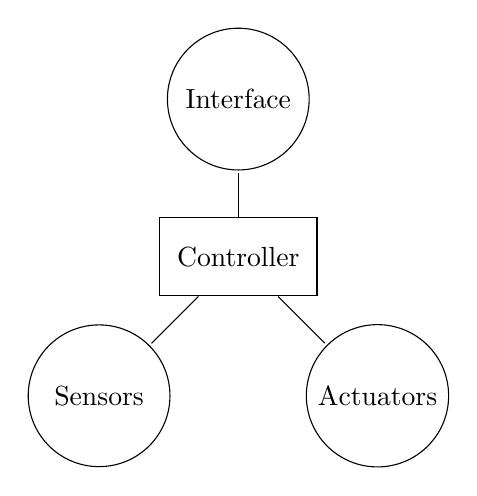
\begin{tikzpicture}[shorten >=1pt,on grid,auto]
	\node[rectangle, draw, scale=1, minimum width=2cm,minimum height=1cm](0) []{Controller};
	\node[circle, draw,node distance=2.0cm, minimum size=1.8cm](1) [above of=0]{Interface};
   	\node[circle, draw,node distance=2.5cm, minimum size=1.8cm](2) [below left of=0]{Sensors};
	\node[circle, draw,node distance=2.5cm, minimum size=1.8cm](3) [below right of=0]{Actuators};
   	\draw (0) -- (1);
	\draw (0) -- (2);
	\draw (0) -- (3);
\end{tikzpicture}
\captionof{figure}{Sensor-Controller-Actuator Architecture}
\label{fig:Sensor-Controller-Actuator Architecture}
\end{center}~\\
In the case of this subsystem, the breakdown of the components into these types will be as follows:
\begin{itemize}
	\item Sensors - System State
	\begin{itemize}
		\item Calibration sensors (quantity yet to be determined)
	\end{itemize}
	\item Sensors - Interface
	\begin{itemize}
		\item Stop buttons (multiple located throughout machine, quantity yet to be determined)
		\item Move button
		\item Take shot button
	\end{itemize}
	\item Logic
	\begin{itemize}
		\item Motion logic
		\item Current state info
	\end{itemize}
	\item Actuators
	\begin{itemize}
		\item Translational motors ($\times2$)
		\item Rotational motor
		\item Pneumatic end-effector
	\end{itemize}
\end{itemize}
\subsubsection{PC Controller Architecture}
This subsystem will utilize a \textit{Rule-Based} architecture style. This style is well suited to making strategic moves while playing a game with rigid rules constraining actions. In other words, for deciding which shot is the best to take given the current state of table and the rules of the game of pool. This style breaks down the subsystem into four types of modules: an interface, a rule-set,  working memory, and an inference engine. The interface will be where the system gets its input and sends its output. The rule-set is a particular sort of knowledge base that contains the rules constraining the acceptable actions. The working memory is temporary memory used by the subsystem. Lastly, the inference engine is what ties the subsystem together. Its job is to apply the rules appropriately and, using the working memory as a tool, generate the appropriate result to send as output.
\newpage 

In the case of this subsystem, the breakdown of these modules into these types will be as follows:
\begin{itemize}
	\item Interface
	\begin{itemize}
		\item Input -- table state
		\item Output -- specification of shot (position, angle, and force)
	\end{itemize}
	\item Rule-Set
	\begin{itemize}
		\item Rules of pool
		\item Mechanical constraints
		\item Physical constants (i.e. ball weight, table friction, spring constant of table cushions, etc.)
	\end{itemize}
	\item Working Memory
	\begin{itemize}
		\item Table state
		\item Current optimal shot
	\end{itemize}
	\item Inference Engine
	\begin{itemize}
		\item Simulate results of shots
		\item Check rules against shot simulations at some incremental angle
		\item Score shots based on weighted application of rules
	\end{itemize}
\end{itemize}
\subsubsection{Camera Architecture}
This subsystem will utilize an \textit{Event-Driven} architectural style. This will likely be the simplest subsystem present in the system. The role of this program is to sit idle waiting for a request to take a picture. Once it receives that request, it should take a picture and then communicate that image back to the PC Controller program. This request is the only event this program must respond to.
\subsubsection{PC VR Program Architecture}
This subsystem will also utilize a \textit{Batch Sequential} architecture style. This style has already been discussed in the system architecture and so will not be discussed again here. In this subsystem, the process is begun upon receipt of the request to start operation. The subsystem will then utilize a VR library to detect the balls as objects on the table using the image provided. The results of this will be passed to the next step which will use the positions of the identified objects to determine which specific ball is which using colour comparison. Once this step completes, the table state has been computed and is then sent back to the PC Controller program. The issues of low throughput and lack of concurrency are not an issue in this case as the system would have to wait for the previous step to complete in order to begin the next step anyway.\\~\\

An illustration of the specific implementation of this architecture is provided below:\\~\\
$$\text{in } \xrightarrow{\text{image}} \text{ object detection } \overset{\text{image \&}}{\xrightarrow{\text{object positions}}} \text{ ball identification } \xrightarrow{\text{table state}} \text{ out}$$
\captionof{figure}{PC VR Architecture}
\label{fig:PC VR Architecture}
\subsection{Likely Changes}
Due to the nature of this project and the condensed time frame in which the development team must produce a prototype, certain aspects in this document are likely to change. Firstly, regarding the physics engine, various physical constants require the system be complete in order to be accurately measured. Currently, any marked TBM are filled with estimated ``placeholder'' values. Also, the method of determining the parallel velocity component after a ball-wall collision should be improved. Secondly, regarding inter-program communication, either a module to adapt given the user's internet settings or a different method of communication would likely be necessary to improve the modularity of the system.



\section{Class Responsibility Collaboration (CRC) Cards}
This section provides CRC cards for all classes in each of the programs. Each card will list the responsibilities as well as any classes the must be collaborated with to perform that responsibility.
\subsection{$\mu$C CRC Cards}
The following are the CRC cards for the $\mu$C program:\\
\begin{table}[!htbp]
\centering
\begin{tabular}{| p{0.5\textwidth} | p{0.3\textwidth} |}\hline
	\multicolumn{2}{|l|}{}\\
	\multicolumn{2}{|c|}{\large{\textbf{SensorMonitor}}}\\
	\multicolumn{2}{|l|}{}\\\hline
	\vspace{0mm}\large{Responsibilities}\vspace{2mm} &\vspace{0mm}\large{Collaborators}\vspace{2mm}\\\hline
	\vspace{0mm}- Sensing signals from buttons	&\vspace{0mm}(None)\\&\\
	- Sensing signals from calibration sensors\vspace{2mm}	&(None)\vspace{2mm}\\\hline
\end{tabular}
\end{table}

\begin{table}[!htbp]
\centering
\begin{tabular}{| p{0.5\textwidth} | p{0.3\textwidth} |}\hline
	\multicolumn{2}{|l|}{}\\
	\multicolumn{2}{|c|}{\large{\textbf{Communicator}}}\\
	\multicolumn{2}{|l|}{}\\\hline
	\vspace{0mm}\large{Responsibilities}\vspace{2mm} &\vspace{0mm}\large{Collaborators}\vspace{2mm}\\\hline
	\vspace{0mm}- Send shot calculation request to the PC Controller Program	&\vspace{0mm}Communicator (PC)\\&\\
	- Receive request receipt confirmation from PC Controller Program			&Communicator (PC)\\&\\
	- Send shot receipt confirmation to PC Controller Program					&Communicator (PC)\\&\\
	- Receive shot specification from PC Controller Program\vspace{2mm}			&Communicator (PC)\vspace{2mm}\\\hline
\end{tabular}
\end{table}

\begin{table}[!htbp]
\centering
\begin{tabular}{| p{0.5\textwidth} | p{0.3\textwidth} |}\hline
	\multicolumn{2}{|l|}{}\\
	\multicolumn{2}{|c|}{\large{\textbf{SignalGenerator}}}\\
	\multicolumn{2}{|l|}{}\\\hline
	\vspace{0mm}\large{Responsibilities}\vspace{2mm} &\vspace{0mm}\large{Collaborators}\vspace{2mm}\\\hline
	\vspace{0mm}- Control translational motors		&\vspace{0mm}Shot Interpreter\\&\\
	- Control rotational motor						&Shot Interpreter\\&\\
	- Control pneumatic end-effector\vspace{2mm}	&Shot Interpreter\vspace{2mm}\\\hline
\end{tabular}
\end{table}
\newpage

\begin{table}[!htbp]
\centering
\begin{tabular}{| p{0.5\textwidth} | p{0.3\textwidth} |}\hline
	\multicolumn{2}{|l|}{}\\
	\multicolumn{2}{|c|}{\large{\textbf{ShotInterpreter}}}\\
	\multicolumn{2}{|l|}{}\\\hline
	\vspace{0mm}\large{Responsibilities}\vspace{2mm} &\vspace{0mm}\large{Collaborators}\vspace{2mm}\\\hline
	\vspace{0mm}Translate shot instruction into list of appropriate signals 	&\vspace{0mm}State, Communicator ($\mu$C)\vspace{2mm}\\\hline
\end{tabular}
\end{table}

\begin{table}[!htbp]
\centering
\begin{tabular}{| p{0.5\textwidth} | p{0.3\textwidth} |}\hline
	\multicolumn{2}{|l|}{}\\
	\multicolumn{2}{|c|}{\large{\textbf{State}}}\\
	\multicolumn{2}{|l|}{}\\\hline
	\vspace{0mm}\large{Responsibilities}\vspace{2mm} &\vspace{0mm}\large{Collaborators}\vspace{2mm}\\\hline
	\vspace{0mm}Store and allow access to data regarding the current physical position of the machine	&\vspace{0mm}Communicator ($\mu$C)\vspace{2mm}\vspace{2mm}\\\hline
\end{tabular}
\end{table}

\begin{table}[!htbp]
\centering
\begin{tabular}{| p{0.5\textwidth} | p{0.3\textwidth} |}\hline
	\multicolumn{2}{|l|}{}\\
	\multicolumn{2}{|c|}{\large{\textbf{Controller}}}\\
	\multicolumn{2}{|l|}{}\\\hline
	\vspace{0mm}\large{Responsibilities}\vspace{2mm} &\vspace{0mm}\large{Collaborators}\vspace{2mm}\\\hline
	\vspace{0mm}Interrupt operation if that instruction is received	&\vspace{0mm}SensorMonitor \\&\\
	Control flow of program operation\vspace{2mm}	&(None)\vspace{2mm}\\\hline
\end{tabular}
\end{table}
\newpage

\subsection{PC Controller CRC Cards}
The following are the CRC cards for the PC Controller program:\\
\begin{table}[!htbp]
\centering
\begin{tabular}{| p{0.5\textwidth} | p{0.3\textwidth} |}\hline
	\multicolumn{2}{|l|}{}\\
	\multicolumn{2}{|c|}{\large{\textbf{Communicator}}}\\
	\multicolumn{2}{|l|}{}\\\hline
	\vspace{0mm}\large{Responsibilities}\vspace{2mm} &\vspace{0mm}\large{Collaborators}\vspace{2mm}\\\hline
	\vspace{0mm}- Listens for request from $\mu$C	&\vspace{0mm}Communicator ($\mu$C)\\&\\
	- Sends confirmation of receipt to $\mu$C		&Communicator ($\mu$C)\\&\\
	- Sends shot specification to $\mu$C			&Communicator ($\mu$C), Shot, Vector\\&\\
	- Listen for receipt confirmation from $\mu$C	&Communicator ($\mu$C)\\&\\
	- Sends image capture request to camera			&EventHandler\\&\\
	- Listens for response from camera				&EventHandler\\&\\
	- Initiate the PC VR program					&(None)\\&\\
	- Read table state from file\vspace{2mm}		&(None)\vspace{2mm}\\\hline
\end{tabular}
\end{table}

\begin{table}[!htbp]
\centering
\begin{tabular}{| p{0.5\textwidth} | p{0.3\textwidth} |}\hline
	\multicolumn{2}{|l|}{}\\
	\multicolumn{2}{|c|}{\large{\textbf{Vector}}}\\
	\multicolumn{2}{|l|}{}\\\hline
	\vspace{0mm}\large{Responsibilities}\vspace{2mm} &\vspace{0mm}\large{Collaborators}\vspace{2mm}\\\hline
	\vspace{0mm}- Stores and allows access to an x- and y-component of a vector	&\vspace{0mm}(None)\\\hline
\end{tabular}
\end{table}

\begin{table}[!htbp]
\centering
\begin{tabular}{| p{0.5\textwidth} | p{0.3\textwidth} |}\hline
	\multicolumn{2}{|l|}{}\\
	\multicolumn{2}{|c|}{\large{\textbf{Ball}}}\\
	\multicolumn{2}{|l|}{}\\\hline
	\vspace{0mm}\large{Responsibilities}\vspace{2mm} &\vspace{0mm}\large{Collaborators}\vspace{2mm}\\\hline
	\vspace{0mm}- Store and allow access to its position							&\vspace{0mm}Vector\\&\\
	- Store and allow access to the value representing its identity\vspace{2mm}		&(None)\vspace{2mm}\\\hline
\end{tabular}
\end{table}
\newpage

\begin{table}[!htbp]
\centering
\begin{tabular}{| p{0.5\textwidth} | p{0.3\textwidth} |}\hline
	\multicolumn{2}{|l|}{}\\
	\multicolumn{2}{|c|}{\large{\textbf{Shot}}}\\
	\multicolumn{2}{|l|}{}\\\hline
	\vspace{0mm}\large{Responsibilities}\vspace{2mm} &\vspace{0mm}\large{Collaborators}\vspace{2mm}\\\hline
	\vspace{0mm}- Store and allow access to the position from which to take this shot	&\vspace{0mm}Vector\\&\\
	- Store and allow access to the angle from which to take this shot					&(None)\\&\\
	- Store and allow access to the amount of power to use to take this shot			&(None)\\&\\
	- Store and allow access to the scoring assigned to this shot\vspace{2mm}			&(None)\vspace{2mm}\\\hline
\end{tabular}
\end{table}

\begin{table}[!htbp]
\centering
\begin{tabular}{| p{0.5\textwidth} | p{0.3\textwidth} |}\hline
	\multicolumn{2}{|l|}{}\\
	\multicolumn{2}{|c|}{\large{\textbf{TableState}}}\\
	\multicolumn{2}{|l|}{}\\\hline
	\vspace{0mm}\large{Responsibilities}\vspace{2mm} &\vspace{0mm}\large{Collaborators}\vspace{2mm}\\\hline
	\vspace{0mm}- Store and allow access to the positions of the balls present on the table		&\vspace{0mm}Ball, Vector\\&\\
	- Store and allow access to the number of both types of ball on the table\vspace{2mm}		&Ball\vspace{2mm}\\\hline
\end{tabular}
\end{table}

\begin{table}[!htbp]
\centering
\begin{tabular}{| p{0.5\textwidth} | p{0.3\textwidth} |}\hline
	\multicolumn{2}{|l|}{}\\
	\multicolumn{2}{|c|}{\large{\textbf{SimulationInstance}}}\\
	\multicolumn{2}{|l|}{}\\\hline
	\vspace{0mm}\large{Responsibilities}\vspace{2mm} &\vspace{0mm}\large{Collaborators}\vspace{2mm}\\\hline
	\vspace{0mm}- Maintain the positions and velocities of balls on the table at the current time step	&\vspace{0mm}TableState, Vector\\&\\
	- Update the positions and velocities of balls after one time step									&TableState, Vector\\&\\
	- Keep track of whether there is still movement occurring											&Vector\\&\\
	- Keep track of the scoring of the simulation (of a shot)\vspace{2mm}								&TableState\vspace{2mm}\\\hline
\end{tabular}
\end{table}
\newpage

\begin{table}[!htbp]
\centering
\begin{tabular}{| p{0.5\textwidth} | p{0.3\textwidth} |}\hline
	\multicolumn{2}{|l|}{}\\
	\multicolumn{2}{|c|}{\large{\textbf{InferenceEngine}}}\\
	\multicolumn{2}{|l|}{}\\\hline
	\vspace{0mm}\large{Responsibilities}\vspace{2mm} &\vspace{0mm}\large{Collaborators}\vspace{2mm}\\\hline
	\vspace{0mm}- Calculate the shot to be made		&\vspace{0mm} SimulationInstance,\newline TableState, Shot, Vector\\&\\\hline
\end{tabular}
\end{table}

\subsection{Camera CRC Cards}
The following is the CRC card for the Camera program:\\
\begin{table}[!htbp]
\centering
\begin{tabular}{| p{0.5\textwidth} | p{0.3\textwidth} |}\hline
	\multicolumn{2}{|l|}{}\\
	\multicolumn{2}{|c|}{\large{\textbf{Event Handler}}}\\
	\multicolumn{2}{|l|}{}\\\hline
	\vspace{0mm}\large{Responsibilities}\vspace{2mm} &\vspace{0mm}\large{Collaborators}\vspace{2mm}\\\hline
	\vspace{0mm}- Listen for request from PC Controller	&\vspace{0mm}Communicator (PC)\\&\\
	- Take a photo										&(None)\\&\\
	- Communicate the photo\vspace{2mm}					&Communicator (PC)\vspace{2mm}\\\hline
\end{tabular}
\end{table}

\subsection{PC VR Program CRC Cards}
The following is the CRC card for the PC VR program:\\
\begin{table}[!htbp]
\centering
\begin{tabular}{| p{0.5\textwidth} | p{0.3\textwidth} |}\hline
	\multicolumn{2}{|l|}{}\\
	\multicolumn{2}{|c|}{\large{\textbf{TableStateVR}}}\\
	\multicolumn{2}{|l|}{}\\\hline
	\vspace{0mm}\large{Responsibilities}\vspace{2mm} &\vspace{0mm}\large{Collaborators}\vspace{2mm}\\\hline
	\vspace{0mm}- Read image from a file		&\vspace{0mm}(None)\\&\\
	- Locate balls using VR						&(None)\\&\\
	- Determine ball identities					&(None)\\&\\
	- Write table state to a file\vspace{2mm}	&(None)\vspace{2mm}\\\hline
\end{tabular}
\end{table}
\newpage



\section{Module Guide}
This section discusses the various modules that this system is comprised of. The modules are divided based on which program they belong to. For each module, its responsibilities, secrets, MIS, and MID will be outlined.
\subsection{Camera Modules}
The following is the module contained within the Camera subsystem.
\subsubsection{EventHandler}
\textbf{Responsibilities}
\begin{itemize}
	\item[-] Listen for request from PC Communicator
	\item[-] Take a photo
	\item[-] Communicate photo to PC Communicator
\end{itemize}~\\
\textbf{Secrets}
\begin{itemize}
	\item[-] Picture-taking process
\end{itemize}~\\
\textbf{MIS}\\[2mm]
This module is an always-running program which executes the function of taking a picture and communicating it back to the requesting program. It's only ``input'' is the request to take a picture. While this module is not performing the previous function, it will be listening for a request to be made.
\\\\
\textbf{MID}\\[2mm]
The state chart below provide a succinct depiction of this module's internal design.\\
\begin{center}
	\includegraphics[width=0.3\textwidth]{EventHandlerStateChart.png}
\captionof{figure}{A state chart for the EventHandler module.}
\label{fig:EventHandlerStateChart}
\end{center}~\\

\subsection{PC VR Program Modules}
The following is the module contained within the PC VR subsystem.
\subsubsection{TableStateVR}
\textbf{Responsibilities}
\begin{itemize}
	\item[-] Read image from a file
	\item[-] Locate balls using VR
	\item[-] Determine ball identities
	\item[-] Write table state to a file
\end{itemize}~\\
\textbf{Secrets}
\begin{itemize}
	\item[-] Object detection algorithm
	\item[-] Ball identification algorithm
\end{itemize}~\\
\textbf{MIS}\\[2mm]
This module takes in an image of a pool table and analyzes it in order to return the locations and identities of each of the pool balls on the table. This is returned in the form of an output file where the n\textsuperscript{th} line contains the x- and y-coordinates for the n\textsuperscript{th} ball.
\\\\
\textbf{MID}\\[2mm]
This module has 4 main steps. First it must read in the image from a predetermined file location. Then it locates the pool balls in that picture using a Visual Recognition object detection algorithm (supplied by a VR library). Next, it will identify which ball is which according to comparing pixel colours within the detected objects to the colours of different pool balls using a LAB colour space. Lastly it will write these results to a file.\\~\\
The following pseudocode better describes this process:
\begin{lstlisting}
read image from file (path to file);
locate balls (image);

for every detected object:
	sample pixels within;
	
	while (pixels not similar to ball archetype AND arcge);
		increment archetype being checked;
		
	if (index out of range):
		raise unidentifiable ball error;
	else:
		results[index for this ball] = this object's location;

return results;
\end{lstlisting}~\\
\begin{center}
	\includegraphics[width=0.175\textwidth]{TableStateVRStateChart.png}
\captionof{figure}{A state chart for the TableStateVR module.}
\label{fig:TableStateVRStateChart}
\end{center}~\\
\subsection{PC Controller Modules}
The following are the modules contained within the PC Controller subsystem.
\subsubsection{InferenceEngine}
\textbf{Responsibilities}
\begin{itemize}
	\item[-] Calculate the best shot to be made
\end{itemize}~\\
\textbf{Secrets}
\begin{itemize}
	\item[-] Algorithm to choose which shots to simulate
	\item[-] The computer's ball type (i.e. stripes or solids)
	\item[-] The rules of pool
\end{itemize}~\\
\textbf{MIS}\\[2mm]
This module allows for specification of a TableState through the use of a 2-D array of doubles. Using that TableState, the module will simulate various potential shots in order to determine an optimal one which is then accessible to other classes in the form of a Shot object.
\\\\
\textbf{MID}\\[2mm]
This module iterates through shots that are to be simulated by SimulationInstances. In order to minimize computation, it only looks at shots that have a hope of directly hitting another legal ball (e.g. the eight ball cannot be struck first unless all of the player's other balls are already sunk). Furthermore, it is assumed that there will only be three discrete power options available to select from. At the end of this computation, this module returns the specification of the optimal shot.\\~\\
The following pseudocode better describes this process:
\begin{lstlisting}
determine balls to shoot;

while (legal balls left to check){
	calculate smallest angle from cue ball to target ball;
	calculate largest angle from cue ball to target ball;
	
	for (all angles from smallest to largest angle){
		for (every power option){
			create SimulationInstance for this shot;
			
			while (simulation not finished){
				simulation.update();
			}
			
			update current shot's score;
			
			if (score of new shot > optimal shot score):
				update optimal shot;
		}		
		current angle += ANGULAR_STEP;
	}
}

return new Shot(calculated X, calculated Y, optimal shot's angle, optimal shot's power);
\end{lstlisting}~\\
\begin{center}
	\includegraphics[width=0.6\textwidth]{InferenceEngineStateChart.png}
\captionof{figure}{A state chart for the InferenceEngine module.}
\label{fig:InferenceEngineStateChart}
\end{center}~\\
\newpage

\subsubsection{PCCommunicator}
\textbf{Responsibilities}
\begin{itemize}
	\item[-] Listens for request from $\mu$C
	\item[-] Sends confirmation of receipt to $\mu$C
	\item[-] Sends shot specification to $\mu$C
	\item[-] Listens for confirmation of receipt from $\mu$C
	\item[-] Sends image capture request to camera
	\item[-] Listens for response from camera
	\item[-] Initiate the PC VR program
	\item[-] Read table state from file
\end{itemize}~\\
\textbf{Secrets}
\begin{itemize}
	\item[-] Receipt confirmation message contents
	\item[-] Maximum time awaiting a response
\end{itemize}~\\
\textbf{MIS}\\[2mm]
This module is an always-running process which communicates with the various programs in this system while also providing control flow for the PC Controller program. The only ``inputs'' it receives is requests from the $\mu$C program and its ``output'' is the shot specification
\\\\
\textbf{MID}\\[2mm]
The state charts below provide a succinct depiction of this module's internal design.
\\\\
\subsubsection{SimulationInstance}
\textbf{Responsibilities}
\begin{itemize}
	\item[-] Maintain the positions and velocities of the balls on the table at the current time step
	\item[-] Update the positions and velocities of the balls on the table after a time step
	\item[-] Keep track of whether there is still movement happening
	\item[-] Keep track of the scoring of the simulation (of a shot)
\end{itemize}~\\
\textbf{Secrets}
\begin{itemize}
	\item[-] The method of calculating a shot's score
	\item[-] Shot simulation algorithm
	\item[-] Physical constants
	\item[-] Simulation time step
\end{itemize}~\\
\textbf{MIS}\\[2mm]
This module handles the physics simulation involved with taking a shot while also scoring the shot according to various criteria. It receives a 2-D array of doubles as ball positions, a double for the angle of the shot, and a double for the power of the shot. These inputs define the initial state of the physical system to simulate. The state is updated for a new time step by calling the appropriate command and an integer representing the resulting change in score from that time step is returned. The Once it returns \textit{false}, there is no further motion and the simulation is complete.
\\\\
\textbf{MID}\\[2mm]
This module handles performing a discrete time step simulation of a shot according to a shot and initial state of the table. In order to achieve this, it updates to the next snapshot of the simulation until every ball remaining on the table is stationary.\\~\\
First, the following pseudocode describes how this object is created:
\begin{lstlisting}
Given:
	An array of balls
	The x and y components of the cue ball's initial velocity
	
inMotion = true;
score = 0;

Initialize the velocities array;

velocities[Ball.CUE__NUM][0] = initial x component;
velocities[Ball.CUE__NUM][1] = initial y component;
\end{lstlisting}~\\\\
The following pseudocode assumes a very fine time step but may not not be feasible given the imposed time constraints (which will be tested empirically):
\begin{lstlisting}
for (all balls on table){
	update position according to velocity;
	update velocity according to friction;
}

for (all balls on table){
	if (in pocket AND sufficiently slow){
		if (cue ball):
			score reduced;
		else if (8 ball AND not shooting 8):
			score reduced;
		else if (wrong type):
			score reduced;
		else:
			score increased;
			
		set position to be off table;
		set velocity to 0;
	}else{
		for (current ball to last ball){
			if (collision):
				compute resulting velocities;
		}
}

for (all balls on table){
	if (velocity != 0){
		inMotion = true;
		return inMotion;
	}
}
\end{lstlisting}~\\
\begin{center}
	\includegraphics[width=0.9\textwidth]{PCCommunicatorStateChart.png}
\captionof{figure}{A state chart for the PCCommunicator module.}
\label{fig:PCCommunicatorStateChart}
\end{center}~\\
\subsection{$\mu$C Modules}
The following are the modules contained within the $\mu$C subsystem.
\subsubsection{Controller}
\textbf{Responsibilities}
\begin{itemize}
	\item[-] Control flow of program operation
	\item[-] Interrupt operation if cancel instruction is received
\end{itemize}~\\
\textbf{Secrets}
\begin{itemize}
	\item[-] Set movement positions (for ``move'' commands)
	\item[-] Instruction dispatch process
\end{itemize}~\\
\textbf{MIS}\\[2mm]
This module handles the control flow for the $\mu$C Program including determining appropriate movement and creation of interrupts when necessary. Its ``inputs'' are when it is notified of state changes such as button presses or position updates from the Sensor Monitor or Signal Generator modules as well as shot specifications (doubles holding the x- and y-coordinates, angle, and power) from the Communicator. Its ``outputs'' are sending the shot request to the Communicator as well as passing on the shot specification to the Signal Generator.
\\\\
\textbf{MID}\\[2mm]
The state chart below provides a succinct depiction of most of this module's internal design. The only other notable component in this module is how it selects where to move when a ``move'' command is received. In that event, it compares the current location to the two set locations at either end of the table. Whichever one is furthest is the one which the machine is moved towards. This is designed in a way such that the machine moves as far away as possible from where it was in the way of the user.~\\
\begin{center}
	\includegraphics[width=0.6\textwidth]{ControllerStateChart.png}
\captionof{figure}{A state chart for the Controller module.}
\label{fig:ControllerStateChart}
\end{center}~\\

\subsubsection{SensorMonitor}
\textbf{Responsibilities}
\begin{itemize}
	\item[-] Sensing signals from buttons
	\item[-] Sensing signals from calibration sensors
\end{itemize}~\\
\textbf{Secrets}
\begin{itemize}
	\item[-] The method of noticing signals
\end{itemize}

\textbf{MIS}\\[2mm]
This module monitors the control signals coming from the buttons and calibration sensors and notifies the Controller when one of these sensors are activated. It's ``inputs'' are the control signals and its ``outputs'' are flags that are raised.
\\\\
\textbf{MID}\\[2mm]
The state chart below provides a succinct depiction of this module's internal design.\\
\begin{center}
	\includegraphics[width=0.4\textwidth]{SensorMonitorStateChart.png}
\captionof{figure}{A state chart for the SensorMonitor module.}
\label{fig:SensorMonitorStateChart}
\end{center}~\\

\subsubsection{ShotInterpreter}
\textbf{Responsibilities}
\begin{itemize}
	\item[-] Translate shot instruction into list of appropriate signals
	\item[-] Control translational motors
	\item[-] Control rotational motor
	\item[-] Control pneumatic end-effector
\end{itemize}~\\
\textbf{Secrets}
\begin{itemize}
	\item[-] Algorithm to determine appropriate movement
	\item[-] Method of transmitting signals to machine
\end{itemize}~\\
\textbf{MIS}\\[2mm]
This module receives a shot specification (doubles holding the x- and y-coordinates, angle, and power) in order to compute and generate the signals necessary to have the machine perform the required motion. It's ``outputs'' are the control signals that it generates.
\\\\
\textbf{MID}\\[2mm]
The state chart below provides a succinct depiction of this module's internal design.\\
\begin{center}
	\includegraphics[width=0.8\textwidth]{ShotInterpreterStateChart.png}
\captionof{figure}{A state chart for the ShotInterpreter module.}
\label{fig:ShotInterpreterStateChart}
\end{center}~\\

\subsubsection{$\mu$CCommunicator}
\textbf{Responsibilities}
\begin{itemize}
	\item[-] Send shot calculation request to the PC Controller program
	\item[-] Receive confirmation of receipt from PC Controller program
	\item[-] Receive shot specification from PC Controller program
	\item[-] Send confirmation of receipt to PC Controller program 
\end{itemize}~\\
\textbf{Secrets}
\begin{itemize}
	\item[-] Receipt confirmation message contents
	\item[-] Maximum time awaiting a response
\end{itemize}~\\
\textbf{MIS}\\[2mm]
This module handles communicating with the PC Controller Program in order to compute the optimal shot to take. It's ``inputs'' are the request from the Controller and the shot specification (doubles holding the x- and y-coordinates, angle, and power) from the PC. It then passes that shot specification on to the Controller.
\\\\
\textbf{MID}\\[2mm]
The state charts below provide a succinct depiction of this module's internal design.\\
\begin{center}
	\includegraphics[width=0.35\textwidth]{uCCommunicatorStateChart.png}
\captionof{figure}{A state chart for the $\mu$CCommunicator module.}
\label{fig:uCCommunicatorStateChart}
\end{center}~\\



\section{Program Diagrams}
\subsection{Detailed Class Diagram}~\\
\begin{sidewaysfigure}
	\begin{center}
		\includegraphics[width=\textwidth]{DetailedClassDiagram.png}
	\captionof{figure}{The system's detailed class diagram.}
	\label{fig:detailedClassDiagram}
	\end{center}
\end{sidewaysfigure}
\newpage

\subsection{Uses Hierarchy Diagrams}
The following section contains the uses hierarchy diagrams for each program.
\begin{center}
	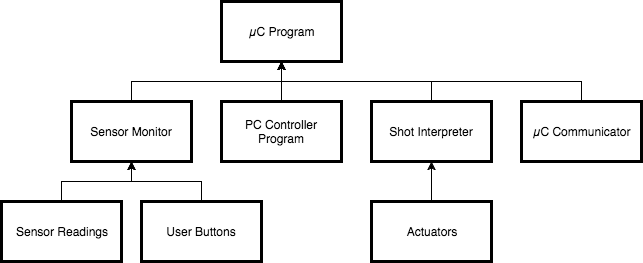
\includegraphics[scale = 0.75]{uCUsesHierarchy.png}
\captionof{figure}{$\mu$C Program Uses Hierarchy Diagram}
\label{fig:ucuses hierarchy diagram}
\end{center}~\\
\begin{center}
	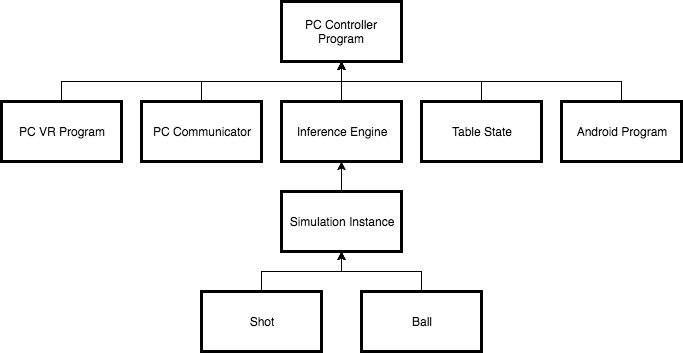
\includegraphics[scale = 0.75]{PCControllerUsesHierarchy.png}
\captionof{figure}{PC Controller Program Uses Hierarchy Diagram}
\label{fig:pc controller uses hierarchy diagram}
\end{center}~\\
\begin{center}
	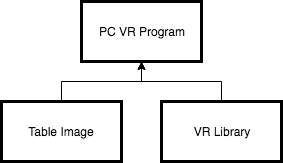
\includegraphics[scale = 0.75]{PCVRUsesHierarchy.png}
\captionof{figure}{PC VR Program Uses Hierarchy Diagram}
\label{fig:pc vr uses hierarchy diagram}
\end{center}~\\
\begin{center}
	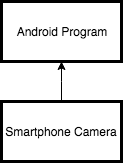
\includegraphics[scale = 0.75]{AndroidUsesHierarchy.png}
\captionof{figure}{Android Program Uses Hierarchy Diagram}
\label{fig:android uses hierarchy diagram}
\end{center}~\\

\subsection{Analysis Class Diagrams}
The following section contains the analysis class diagrams for the $\mu$C and the PC Controller program. The PC VR program and Camera are not complicated enough to require the inclusion of these diagrams.\\
\begin{center}
	\includegraphics[scale = 0.75]{muCAnalysisClassDiagram.png}
\captionof{figure}{$\mu$C Analysis Class Diagram}
\label{fig:muC analysis class diagram}
\end{center}~\\
\begin{center}
	\includegraphics[scale = 0.75]{PCControllerAnalysisClassDiagram.png}
\captionof{figure}{PC Controller Analysis Class Diagram}
\label{fig:PC controller analysis class diagram}
\end{center}



\section{Physics Simulations}
A substantial component of this system will be the ability to simulate and score a shot. Scoring will be determined by which balls are sunk (if any).
\subsection{Constants}
The following constants will be used by this system's simulation engine. Certain values must be measured empirically and will be marked To Be Measured (TBM). All values will be in standard SI units.
\begin{center}
\setlength\extrarowheight{5pt}
\begin{tabular}{c | l | c}
	\multicolumn{1}{>{\centering\arraybackslash}c |}{\textbf{Constant}} 
    & \multicolumn{1}{>{\centering\arraybackslash}c |}{\textbf{Description}} 
    & \multicolumn{1}{>{\centering\arraybackslash}c}{\textbf{Value}}\\[-4mm]&&\\\hline
	$C_{R_b}$		&Coefficient of Restitution, ball - ball	&0.96\\
	$C_{R_w}$		&Coefficient of Restitution, ball - wall	&0.866\\
	$g$				&Gravitational Acceleration					&9.807\\
	$v_{i_1}$		&Initial Speed, soft hit					&TBM\\
	$v_{i_2}$		&Initial Speed, medium hit					&TBM\\
	$v_{i_3}$		&Initial Speed, hard hit					&TBM\\
	$\mu_k$			&Kinetic Friction, ball - cloth				&TBM\\
	$m_b$			&Mass, ball									&0.163\\
	$v_{sink}$		&Maximum Speed to Sink Ball					&TBM\\
	$x_{max}$		&Maximum x-coordinate						&1.848\\
	$y_{max}$		&Maximum y-coordinate						&0.921\\
	$r_{ball}$		&Radius (ball)								&0.0286\\
	$\mu_s$			&Static Friction, ball - cloth				&TBM\\
	$T$				&Time Step									&0.01\\
	$w_c$			&Width, mouth of corner pocket				&0.1\\
	$w_s$			&Width, mouth of side pocket				&0.114
\end{tabular}
\end{center}
\subsection{Equations}
The program will utilize the following equations to predict the evolution of the simulation.\\[4mm]
\textbf{Ball - Ball Collision}\\
{\large
\begin{align*}
	v_{a_f}	&= \frac{C_{R_b}m_b(v_{a_i} - v_{b_i}) + m_av_{a_i} + m_bv_{b_i}}{m_a + m_b}
\end{align*}
}
Since the masses are equivalent, this simplifies to..
{\large
\begin{align}
	v_{a_f}	&= \frac{1}{2}(C_{R_b}(v_{b_i} - v_{a_i}) + v_{a_i} + v_{b_i})
\end{align}
}\\
\textbf{Ball - Wall Collision (perpendicular component)}%TODO
{\large
\begin{align}
	v_f	&= -C_{R_w}v_i
\end{align}
}\\
\textbf{Ball - Wall Collision (parallel component)}
{\large\\~\\[-2mm]
Currently, this equation will not affect the velocity of the balls however this is just a simplification and is likely to be altered.
\begin{align}
	v_f	&= v_i
\end{align}
}\\
\textbf{Ball Velocity Update}
{\large
\begin{align}
	v_f	&= v_i \cdot \mu_k \cdot T
\end{align}
}\\
\textbf{Ball Position Update}
{\large
\begin{align}
	d_f	&= d_i + vT
\end{align}
}\\



\section{Communication Protocols}
This section will outline the protocols used for communicating between the various devices and programs within this system. This is crucial as the different programs will rely on standard formats in order to understand the contents of messages.
\subsection{$\mu$C - PC Controller}
These programs must both be able to communicate message receipts, the $\mu$C must be able to make a shot request to the PC Controller, and the PC Controller program must be able to send shot specifications back to the $\mu$C. The receipts will be very simple messages, just containing an unsigned integer byte with the value 200. The shot request will also be an unsigned integer byte holding the value 55. Lastly, the shot specification will be sent as follows:
\begin{center}
	170, x, y, angle, power
\end{center}
where the number 170 is stored as an unsigned integer byte, x and y are the coordinates for the shot in double-precision floating point (8 bytes), angle is the angle of the shot in double-precision floating point, and power is the power of the shot stored in a single byte (either 1, 2, or 3).\\\\
The various numbers at the beginning of messages act as both checksums and indicators of the message's contents. The numbers were chosen purposefully in a manner such that they have very different one byte binary representations (they share at most 4 common digits).\\\\
Communication will occur wirelessly using either bluetooth or Wi-Fi as determined by availability of hardware and software resources.
\subsection{PC VR - PC Controller}
The PC VR program must be able to communicate the table state to the PC Controller. This will be accomplished by writing results to a file with the following format:
\begin{center}
	Cue Ball x-coordinate, Cue Ball y-coordinate\\
	1 Ball x-coordinate, 1 Ball y-coordinate\\
	2 Ball x-coordinate, 2 Ball y-coordinate\\
	~\vdots\\
	15 Ball x-coordinate, 15 Ball y-coordinate
\end{center}
where each set of coordinates is separated by a newline character and there are exactly 16 lines.
\subsection{Camera - PC Controller}
The PC Controller must be able to request a picture be taken and the camera must be able to communicate the image back to the PC Controller. Similar to the protocol between the $\mu$C and the PC Controller, the request will be a single unsigned integer byte holding the value 55 and the image data being sent will be preceded by a single unsigned integer byte holding the value 170. As mentioned previously, these values will act as checksums.



\section{Scheduling of Tasks}
The goal of this section is to outline the ordering and maximum allowable time frames of tasks in this program.
\subsection{Allocation of Time}
From the requirements document, there is only 90 seconds allowed between pressing a button and a shot being made. The most difficult computational step will be the shot simulations and so this section will deduce how much time the machine will have for that step.\\~\\
Firstly we must account for how long the physical machine would need in the worst case (moving all the way across both axes and rotating 180 degrees). To be fair, we will allocate 20 seconds to this operation.\\~\\
From here we can divvy up the remaining time among the various computational blocks. The smaller tasks such as communication, recognizing the button press, and other such operations will be allocated a total of 5 seconds. The process of object detection and identification will be given 15 seconds. This leaves 50 seconds to process the necessary simulations.

\subsection{Sequence Diagrams}
The following are various sequence diagrams for different actions the system is required to perform. These diagrams are meant to provide better context for how the classes interact with each other to perform certain tasks.\vfill
\begin{center}
	\includegraphics[width=0.6\textwidth]{MoveSequenceDiagram.png}
\captionof{figure}{A sequence diagram for the ``move'' operation.}
\label{fig:MoveSequenceDiagram}
\end{center}
~\vfill
\begin{center}
	\includegraphics[width=0.6\textwidth]{cancelSequenceDiagram.png}
\captionof{figure}{A sequence diagram for the ``cancel'' operation.}
\label{fig:CancelSequenceDiagram}
\end{center}
~\vfill

\begin{sidewaysfigure}
	\begin{center}
		\includegraphics[width=\textwidth]{TakeShotSequenceDiagram.png}
	\captionof{figure}{A sequence diagram for the ``take shot'' operation.}
	\label{fig:TakeShotSequenceDiagram}
	\end{center}
\end{sidewaysfigure}
\end{document}

